\chapter{Background}
\label{background}

\section{Glycosaminoglycans (GAGs)}
\label{background:gags}


\subsubsection{General aspects}%The nature of GAGs}
Carbohydrates are ubiquitous building blocks found in all forms of life. As
implicated by their name, they are made of carbon, hydrogen and oxygen. Despite
this rather small set of atom types, an enormous variety of carbohydrates
exists. The origin of major parts of this diversity is of combinatorial nature:
carbohydrates usually occur as polysaccharides made of many connected
monosaccharides (or \enquote{sugar rings}), whereas various different types of
monosaccharides are available in nature. They are distinguishable by their
chemical configuration, and usually there are two stereoisomers for each of
those configurations, leading to a broad spectrum of different sugar rings whose
nomenclature and chemistry are described in detail in reference books
\cite{carbohydrate_chemistry_robyt_1998, carbohydrate_chemistry_royal_2000}.
Glycosaminoglycans (GAGs), reviewed in
\cite{essentials_glycobiology_gags_chapter_2009}, are a special class of
carbohydrates. GAGs play a critical role in many biological processes; they are
important for cell adhesion and cell growth, and their multifarious biological
activity arises from their ability to interact with and regulate a large number
of proteins \cite{handel_2005,gandhi_structure_2008}. Likewise, both natural and
artificial GAGs are promising tools for therapies, for instance for the design
of new bio-materials for the use in the field of regenerative medicine
\cite{whitelock_2014,schnabelrauch_tissues_2013,scott_gags_therapies_2013}.

GAGs are unbranched (linear) saccharide chains, comprised of a periodically
repeating unit, whereas each unit is made of two pyranose (a six-membered ring
consisting of five carbon atoms and one oxygen atom) monosaccharides:

\nomenclature{GAG}{glycosaminoglycan}

\begin{itemize}
\item One is an amino sugar or \enquote{hexosamine}, either a
D\-/N\-/acetylglucosamine (GlcN) or a D\-/N\-/acetylgalactosamine (GalN).
\item The other is a uronic saccharide or \enquote{hexuronic acid}, either a
D-glucuronic acid (GlcA) or its C5\-/epimer L\-/iduronic acid (IdoA), or, in
seldom cases, a D\-/galactose (Gal).
\end{itemize}


\nomenclature{IdoA}{L-iduronic acid}
\nomenclature{GlcA}{D-glucuronic acid}
\nomenclature{GalN}{D-N-acetylgalactosamine}
\nomenclature{GlcN}{D-N-acetylglucosamine}


\begin{table}
\scriptsize
\centering
\renewcommand{\arraystretch}{1.3}
\begin{tabular}{lll}
\midrule
GAG type & main disaccharide & charge/\si{\elementarycharge} \\
\midrule
Heparin (HP) & L-IdoA2S-$\alpha$(1$\rightarrow$4)-D-GlcNS6S-$\alpha$(1$\rightarrow$4) & -4 \\
Chondroitin-4-sulfate (CS4) & D-GlcA-$\beta$(1$\rightarrow$3)-D-GalN4S-$\beta$(1$\rightarrow$4) & -2 \\
Hyaluronan (HA) & D-GlcA-$\beta$(1$\rightarrow$4)-D-GlcN-$\alpha$(1$\rightarrow$4) & -1 \\
\midrule
\end{tabular}
\caption{
Fundamentally different GAG types, their repeating disaccharide unit in IUPAC
nomenclature, and their charge per disaccharide, in units of the elementary
charge. The abbreviations given in brackets in the first column are used
throughout this thesis.}
\label{tab:bg:gagtypes}
\end{table}

\nomenclature{HP}{heparin}
\nomenclature{HA}{hyaluronan}
\nomenclature{CS4}{chondroitin-4-sulfate}
\nomenclature{CS6}{chondroitin-6-sulfate}

A special feature of GAGs is that they are usually sulfated at various ring
positions, leading to a number of possible sulfation patterns per repeating
disaccharide unit. The number of possible combinations of basic disaccharide
units, two different allowed geometries of the glycosidic linkage between them,
and variations in the sulfation pattern imply that the heterogeneity among GAGs
is large. Still, physiologically occurring GAGs can be roughly categorized into
six major GAG types. Three of those, the most important ones for this thesis,
are listed in \cref{tab:bg:gagtypes} together with their repeating disaccharide
unit, sulfation pattern, glycosidic linkage type, and with their abbreviation
used here from now on. Three other major GAG types are usually listed in
literature \cite{gandhi_structure_2008}, which play a less important role in
this thesis than the ones listed in \cref{tab:bg:gagtypes}:

\begin{itemize}
\item Heparan sulfate, which is considered to be an analogue of heparin. The
only difference is that heparan sulfate has --- on average --- a higher content
of glucuronic acid than iduronic acid.
\item Dermatan sulfate, which is similar to chondroitin sulfate, but is built of
iduronic acid instead of glucuronic acid.
\item Keratan sulfate, the only GAG type that contains a D\-/galactose
saccharide instead of an acid. The amino sugar is the same as in chondroitin
sulfate.
\end{itemize}

Except for HA, which is the only non-sulfated GAG, the naturally occurring
sulfation of GAGs is strong, with up to three sulfate groups per disaccharide
unit in case of heparin. Considering the carboxyl group contained in the
hexuronic acid, each repeating disaccharide unit always carries at least one
negative charge at physiological pH (which is also true for HA). Adding
sulfation, this charge may grow up to -4 for heparin (see
\cref{tab:bg:gagtypes}), which in fact is the biological macromolecule with the
largest charge density known \cite{capila_linhardt_hep_prot_2002}.
\Cref{fig:bg:heparin_chemstruct} shows the chemical configuration of the
repeating disaccharide unit of heparin and schematically visualizes its
structure in space. What is depicted there actually is the disaccharide unit
which occurs \textit{most frequently} in natural heparin polysaccharides.
Polymeric GAGs in an organism can be quite long with a molecular weight of about
10 to 100\,kDa \cite{gandhi_structure_2008}, and they never reach
\SI{100}{\percent} purity. That is, natural GAGs are always comprised of a
mixture of more than only two monosaccharides, and the repeating units shown in
\cref{tab:bg:gagtypes} are the \textit{dominating} ones for each of the cases.

\begin{figure}
\centering
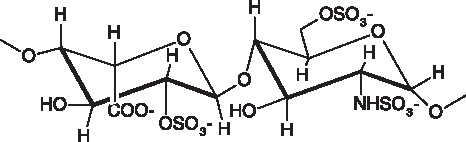
\includegraphics[width=1.0\textwidth]{gfx/background/hp_repeating_unit_structure_01.pdf}
\caption[]{
Molecular configuration of the repeating disaccharide unit of heparin (the one
which occurs most frequently in natural heparin polysaccharides). The pyranose
to the left is a 2-O-sulfated iduronic acid (IdoA2S), connected via a
1$\rightarrow$4 glycosidic linkage to the 6-O-sulfated
2-deoxy-2-sulfamido-α-D-N\-/acetylglucosamine (GlcNS6S). At physiological pH,
the charge of this disaccharide is -4 elementary charges.
}
\label{fig:bg:heparin_chemstruct}
\end{figure}

There are many more than six GAG variants with established names, such as
Chondroitin\-/6\-/sulfate (CS6), which is the same as CS4, but sulfated at the
C6 position of the galactosamine instead of in the fourth position. With the GAG
types described here so far, all major characteristics of naturally occurring
GAG molecules are covered. Other GAG types are not listed, because they are not
fundamentally different from what has been described and therefore were not
investigated in the framework of this thesis.

In organisms, all GAG chains except for HA  appear covalently bound to a core
protein, comprising a so-called \textit{proteoglycan} complex
\cite{essentials_glycobiology_gags_chapter_2009}. These large structures consist
of a linear protein with many GAGs covalently linked to it. Each GAG is linked
to the core protein via a special sugar linker, which itself is attached to
(usually) a serine residue of the core protein. As of the length of the GAG
chains, however, the biological functions of proteoglycans depend to a large
extent only on the interaction of its GAG chain(s) with other proteins, i.e.\
the free end of a GAG chain can be considered unaffected by the core protein.
This is one of the fundamental assumptions applied in this thesis project: GAGs
are considered and treated as \textit{free} molecules.



%While it is likely
%that their tremendous length and also their covalent linkage to proteoglycans
%serve have an overall impact on the biological function of GAGs, it is a
%valid and well-established approximation to not account for these facts in
%molecular modeling studies that aim for resolving the molecular mechanism of
%protein-GAG interaction in atomic detail... in a biological function and overall  treated as


\subsubsection{Pyranose conformations}
\label{background:gags:conformations}

The origin and geometry of various pyranose monosaccharide conformations is
comprehensibly classified and discussed in
\cite{classification_pyranose_conformers_1960}. The conformational nomenclature
used throughout this thesis follows IUPAC rules, which are well-described in
\cite{iupac_gag_conformations_1980}.

Free in solution, most monosaccharide rings in GAGs have one clearly predominant
conformation, and their ring structure can therefore be considered
\textit{rigid}, as is the case for e.g.\ D-glucuronic acid (GlcA), which resides
in a stable ${}^{4}\mathrm{C}_1$ chair \cite{almond_jacs_2010}. Also
N-acetyl-D-glucosamine (GlcN) mainly populates the ${}^{4}\mathrm{C}_1$ ring
conformation, which was shown to be especially stable when the GlcN becomes
sulfated \cite{Sattelle_glcnac_right_chair_2011}, as is the case in heparin. The
pyranose ring of iduronic acid (IdoA), a constituent of heparin, however, is the
only GAG pyranose that is --- free in solution, i.e.\ without any mechanical
stress --- in an equilibrium of multiple so-called ring puckers. C5 carboxyl
epimerization is the the only difference of IdoA compared to GlcA, and it
results in conformational instability. IdoA is postulated to be populated by a
mixture of mainly three conformations \cite{almond_jacs_2010}:
${}^{4}\mathrm{C}_1$, ${}^{1}\mathrm{C}_4$, and ${}^{2}\mathrm{S}_\mathrm{O}$.
Obviously, this conformational flexibility of IdoA is a \textit{structural
flexibility} which allows for different orientations of functional groups in
space, as depicted in \cref{fig:bg:idoa_conformations}.

\begin{figure}
\centering
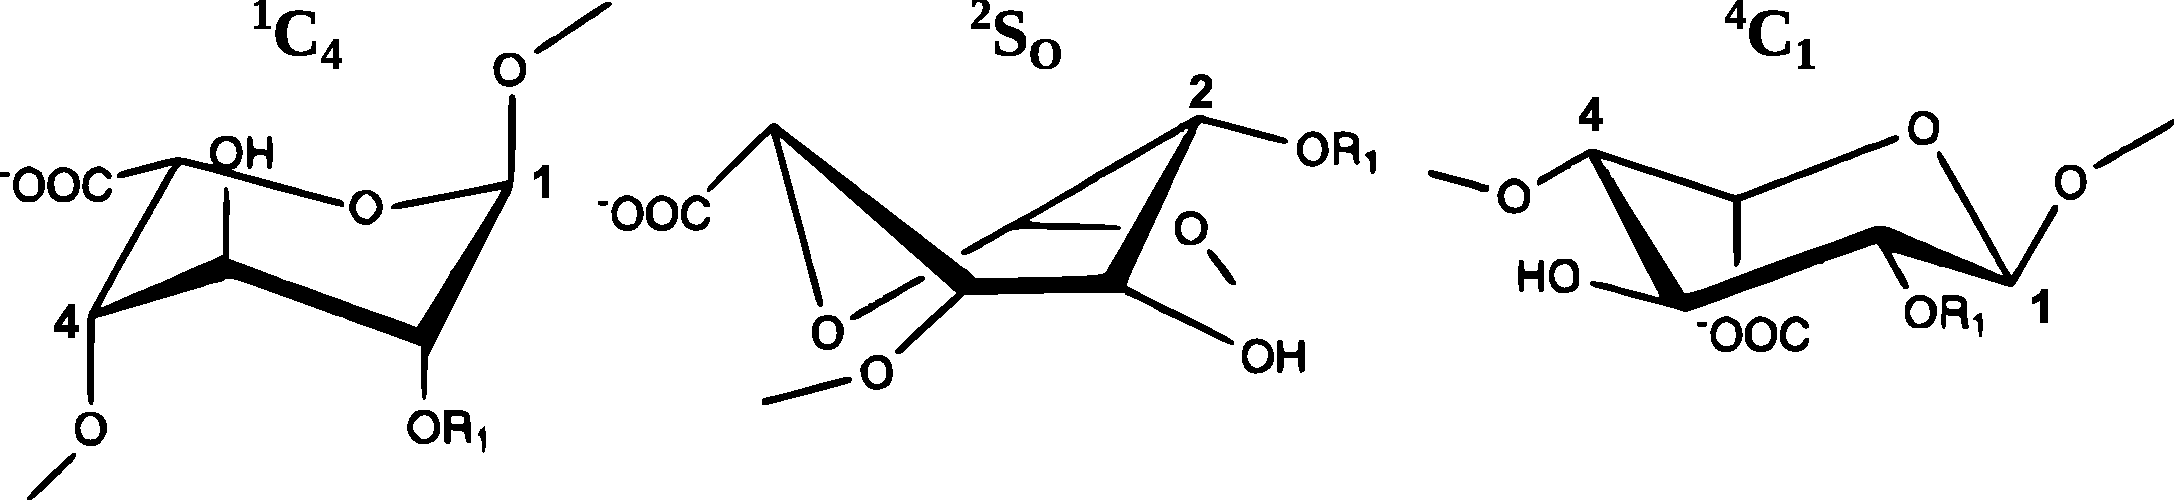
\includegraphics[width=1.0\textwidth]{gfx/background/idoa_conformations_03.pdf}
\caption[]{
The three conformations (two chairs, one skew-boat) of the pyranose L-iduronic
acid which are most populated in solution. In heparin, $\mathrm{R}_1$ is a
sulfate group.}
\label{fig:bg:idoa_conformations}
\end{figure}


The exact population ratios and exchange time scales of the conformations of
IdoA are difficult to measure and simulate \cite{almond_jacs_2010,
structure_gags_progess_perspectives_2010}, but they clearly depend on the IdoA
environment. That is, a terminal IdoA behaves differently from an IdoA pyranose
within a GAG chain. As shown by Sattelle et al., the population ratio depends on
sulfation, and IdoA2S still prevails in an equilibrium of multiple highly
populated conformations \cite{almond_jacs_2010}. Regarding heparin-internal
IdoA2S, Muñoz-García and co-workers summarize that it is in an equilibrium of
${}^{2}\mathrm{S}_\mathrm{O}$ and ${}^{1}\mathrm{C}_4$ with a negligible content
of the ${}^{4}\mathrm{C}_1$ chair \cite{conf_idoa_timeavg_restraints_2013}. The
interconversion between ${}^{2}\mathrm{S}_\mathrm{O}$ and ${}^{1}\mathrm{C}_4$
has earlier been described to exert only little geometrical change on glycosidic
linkages \cite{Mulloy_dyn_conf_heparin_2000}, rendering the overall
polysaccharide conformation independent on iduronic acid ring puckering
\cite{jin_heparin_2009}. Likewise, Gandhi and Mancera conclude that whilst the
spatial orientation of the 2-O-sulfate group in IdoA2S in heparin is altered
during conformation interconversion, no significant structural change can be
seen in the backbone of the polysaccharide chain \cite{gandhi_structure_2008}.


\subsubsection{General aspects about protein-GAG interaction}

It is state of knowledge that GAGs play a critical role in many biological
processes \cite{handel_2005}. In many of these scenarios, GAGs directly interact
with proteins on the molecular level. According to Esko and Linhardt, more than
100 GAG-binding proteins have been described in literature
\cite{essentials_glycobiology_protgags_2009}. To a large extent, the
corresponding studies were focused on protein interaction with heparin only.
Esko and Linhardt speculate that this bias towards heparin may reflect the
commercial availability of heparin and the fact that the interaction between
proteins and heparin can be assumed to properly mimic the physiological
interaction of proteins with heparan sulfate, which is especially abundant on
cell surfaces and in the extracellular matrix. Esko and Linhardt note that
relatively few proteins are known to interact with chondroitin sulfate or
keratan sulfate. However, in some cases, especially chondroitin sulfate's
interaction with proteins may be physiologically relevant, because chondroitin
sulfate is the most abundant GAG in the body
\cite{gandhi_structure_2008} and available in many tissues
\cite{essentials_glycobiology_protgags_2009}.

Several protein-GAG systems of which it is long known that they have huge
biological impact were, in the course of countless studies, investigated via
structural biology methods, biochemically, and via molecular modeling approaches
in order to understand the \textit{molecular basis} of the interaction.
Fundamental findings were especially made with X-ray crystallography and via
nuclear magnetic resonance (NMR), both of which are able to spatially resolve
the arrangement of atoms in the bound state of a protein-GAG complex. However,
NMR and X-ray studies implicate an enormous experimental effort and are often
not successful, so that up to now the number of experimentally obtained
protein-GAG complex structures deposited in the PDB is still quite low
(\hl{about 80}).

% Still, from these well-investigated complexes, a number of
% essential observations is to be made for this thesis work.

The experimentally resolved structures of protein-GAG complexes typically
contain GAG molecules of lengths between dp2 and dp10, with the most common
length being dp5 (\enquote{dp} stands for degree of polymerization, and the
following number is the number of monosaccharides in the molecule). Khan et al.\
argue that HP dp4 possesses a sufficient number of at least six sulfate groups
and two carboxyl groups to generate protein specificity for heparin
\cite{semi_rigid_heparin_structures_2010}. Hence, GAG binding epitopes
responsible for affinity \textit{and} specificity of the protein-GAG interaction
are typically rather short --- at least for the systems contained in the PDB so
far, and a counter-example is yet to be discovered. Likewise, recent
experimental and molecular modeling studies for the investigation of protein-GAG
systems focused on using short GAGs \cite{pichert_characterization_2012,
hintze_sergey_2014, gandhi_coombe_2008, Gandhi01102009,
mancera_gandhi_jcim_2011, agostino_mancera_gandhi_2014}. An important
observation is that in most crystal structures, GAG binding sites are found on
surface-exposed positions, almost always containing positively charged amino
acid residues (at physiological pH, which are arginine and lysine).

Regarding heparin-protein interaction, a number of crystal structures and NMR
experiments suggest that when heparin binds to a protein, the iduronic acid may
undergo an induced fit, and prefer one of its possible ring conformations
\cite{gandhi_structure_2008}. The conformational flexibility of IdoA and
therefore its ability to structurally adjust itself to a protein may be one of
the reasons why many important and high-affinity protein-GAG interactions
involve heparin, and not other GAG types. On the other hand, there are also
protein-GAG complexes for which it has been shown that IdoA in the bound state
can still assume multiple conformations \cite{barbero_jacs_2005}, in which case
the entropy penalty associated with the restriction of single degrees of freedom
would be reduced. Overall, however, the scientific community generally assumes
that heparin's pure charge density is mainly responsible for its seemingly
dominant role in protein-GAG interaction \cite{gandhi_structure_2008,
essentials_glycobiology_protgags_2009}.



\subsubsection{Structure of GAGs}

While the geometry of monosaccharides is well-investigated and in most of the
cases known with an enormous degree of detail, the investigation of the
three-dimensional solution structure of GAG polysaccharides, i.e.\ its overall
flexibility and conformation, is rather unclear and topic of ongoing research
\cite{structure_gags_progess_perspectives_2010}. The GAG structures contained in
the PDB, as stated above, are limited to smaller fragments of not more than 10
monosaccharides. Among these bound structures, GAGs appear to be linear, quite
flexible molecules that do not assume a special secondary structure.
Additionally, Khan et al. found via X-ray scattering and constrained modeling
that longer heparin oligosaccharides (up to dp36) that are free in solution
assume a rather extended semi-rigid conformation
\cite{semi_rigid_heparin_structures_2010}. One of the most important criteria
for characterizing GAG structures are their glycosidic linkage dihedral angles.
In this regard, the X-ray and NMR measurements reported in literature very much
agree on a certain angle interval, which is accessible to all major GAG types,
conceptually comparable to the well-known backbone dihedral angle intervals
which are valid for proteins. Obviously, this kind of data enables us to
estimate whether a certain GAG structure is valid or not, and it also allows us
to quantify the overall backbone flexibility of GAGs. An overview over
literature-reported heparin backbone dihedral angles can be found in e.g.\
\cite{semi_rigid_heparin_structures_2010}.



\section{A primer on IL-10 biology}

 IL-10's biological function is mainly considered to be
, but

 has pleiotropic effects in immunoregulation and
inflammation.


        in closing remarks, relate to extracellular matrix


%\subsubsection{GAG structures used in \textit{in silico} experiments}


Here, or in the section below, quote all from Roers!

\section{IL-10 and its relation to GAGs}


 anti-inflammatory

- Relevance of IL-10 in immune regulation
- Bio-relevant IL-10-GAG interaction? Motivated by Salek ardakini.

We are interested in GAG interaction with the cytokine interleukin-10 (IL-10,
reviewed in \cite{moore_2001}), which is generally considered to exert an
immunosuppressive function. From \textit{in vitro} experiments, IL-10 is known
to bind GAGs and there is evidence that GAGs may modulate its biological
function \cite{salek_ardakani_2000}. So far however, no structural detail about
IL-10-GAG interaction is known.


Wherever IL-10 is supposed to
regulate an immune response, for instance in the process of wound healing and
tissue regeneration, GAGs are


\section{In-silico methods for investigating protein-GAG interaction}


\subsubsection{GAG representation approximations: isolation, length, purity}

As has been stated above, one of fundamental assumptions applied in this thesis
project: GAGs are treated as \textit{free} molecules.

%While it is likely
%that their tremendous length and also their covalent linkage to proteoglycans
%serve have an overall impact on the biological function of GAGs, it is a
%valid and well-established approximation to not account for these facts in
%molecular modeling studies that aim for resolving the molecular mechanism of
%protein-GAG interaction in atomic detail... in a biological function and overall  treated as

A more severe approximation applied in this thesis is the treatment of GAGs as
\textit{short} molecules. Considering the  mostly ranging from tetra- to hexasaccharides. Considering the level of atomic detail aimed for ... to be observed... in this
thesis project, GAGs are modeled as short molecules.


Also, when treating GAGs as short molecules, they are represented by the ideal
periodic repetition of the most frequently observed disaccharide unit,
impurities or variations in the monosaccharide sequence are ignored.

ir ideal periodic

explain DP, degree of polymerization

\nomenclature{dp}{degree of polymerization}



From Sergey: Computationally, GAG containing systems are still very challenging
to handle because of their high flexibility as it applies for saccharides in
general 15, importance of taking into account solvent mediated interactions16,17
and required proper treatment of electrostatics due to their charged nature
1,18,19. For heparin, in addition, the rings of IdoU2S can adopt two pucker
conformations (1C4 and 2S0) with comparable probability 20–23, which, therefore,
can represent a combinatorial task for modeling periodic molecules of heparin,
and which proper consideration is outside the scope of classical MD time scales
and common force fields at the moment 24,25. Nevertheless, both experimental and
computational studies show that even a single IdoU2S ring conformational change
significantly contributes to the specificity of GAG/protein complex formation
both structurally and thermodynamically 26,27. Moreover, it is known
that for relatively big systems like collagen-based matrixes, where interactions
with GAGs could be crucial for their mechanical properties 29–31, application of
the approaches which use only short GAGs does not seem to be proper.



\subsection{A primer on docking methods}


    - Methods applied in literature: a mini review
        AutoDock3 stands out, just by experience, not by concept
    - Problems of different complexity: local vs. global docking.
    - (AutoDock 3 protein-GAG blind docking validation study,
        Method, results, discussion, conclusion)

\lipsum[1-5]

\subsection{A primer on molecular dynamics simulations}

\lipsum[1-5]

\subsubsection{End-point free energy methods (\enquote{MM-PB(GB)SA})}
% This label is required in DMD chapter.
\label{methods:mmpbsa_mmgbsa}


Cite this: \cite{schlick_innovationsdynamics_2012} (volume 2, chapter 12).

\lipsum[1-5]

\section{Structure of the IL-10 system}

    - Structure description
        exists mainly as homodimer [
            biochemistry, 1998, 37, 16943-16951, zdanov 1995]


    - IL-10 and its receptors
        - what is known in literature (current state of knowlege)
            R1+IL-10 structure
            R2 structure
            ternary complex binding models
            what is required for signaling? literature overview
        - a critical review: monomer
            minimal unit required for signaling (monomer)
        - IL-10 + R1 + R2 structure model from IL20 ternary complex


\section{Aim and scope of this thesis}

- Vision: gaining control over IL-10 function in artificial extracellular matrices

- Motivation and goal: investigate IL-10-GAG system with computational
      methods, in collaboration with...

The aim of this project is to unravel atomic details of IL-10-GAG interaction
with theoretical and computational means. If required, methodological approaches
are to be developed. Integration of \textit{in silico}-based predictions with
experimental results from collaborators will hopefully provide insights into the
mechanisms determining IL-10-GAG interaction. Methodology developed during this
project is applicable to protein-GAG systems in general, rendering it valuable
for a large field of research.



\hl{cite interleukin-2 -heparin interaction (mulloy, rider) !}

\lipsum[1-5]





